%!TEX root = ../thesis.tex

\chapter{Introduction}
\label{sec:introduction}


This is a complete template for the MSc Geomatics thesis.
It contains all the parts that are required and is structured in such a way that most/all supervisors expect.
Observe that the MSc Geomatics at TU Delft has no requirements, so I took the liberty of formatting it the way I like. 
Well, I simply took the template \texttt{arsclassica} (by Lorenzo Pantieri), which is an adaption of the original \texttt{classicthesis} package from André Miede, and structured it in such a way that all sections are present.

\emph{It is not an official template and it is not mandatory to use it.}

But I hope it will encourage everyone the use of \LaTeX, and I also hope that it will discourage students to use Word\ldots

If you run into mistakes/problems/issues, please report them on the GitHub page, and if you fix an error, then please submit a pull request. 

\url{https://github.com/tudelft3d/MScGeomaticsThesisTemplate}.



\section{Figures}

\begin{figure}
  \centering
  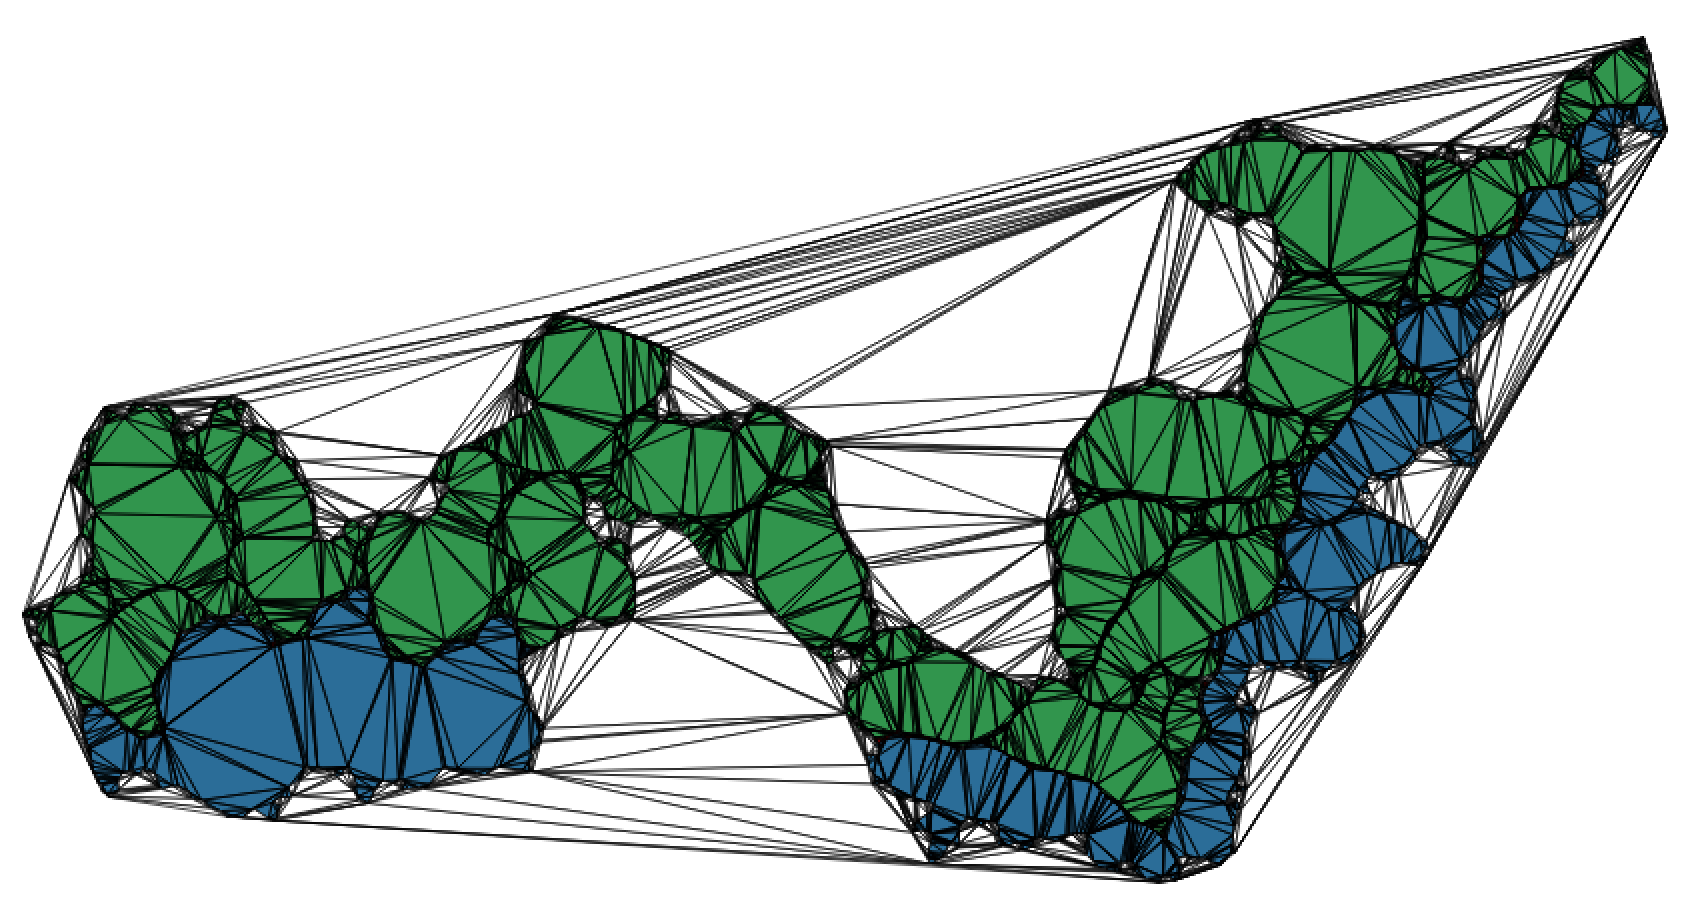
\includegraphics[width=0.8\linewidth]{figs/sometriangles.png}
  \caption{One nice figure}
\label{fig:sometriangles}
\end{figure}

As shown in Figure~\ref{fig:sidebyside},
\begin{figure}
  \centering
  \begin{subfigure}[b]{0.45\linewidth}
    \centering
    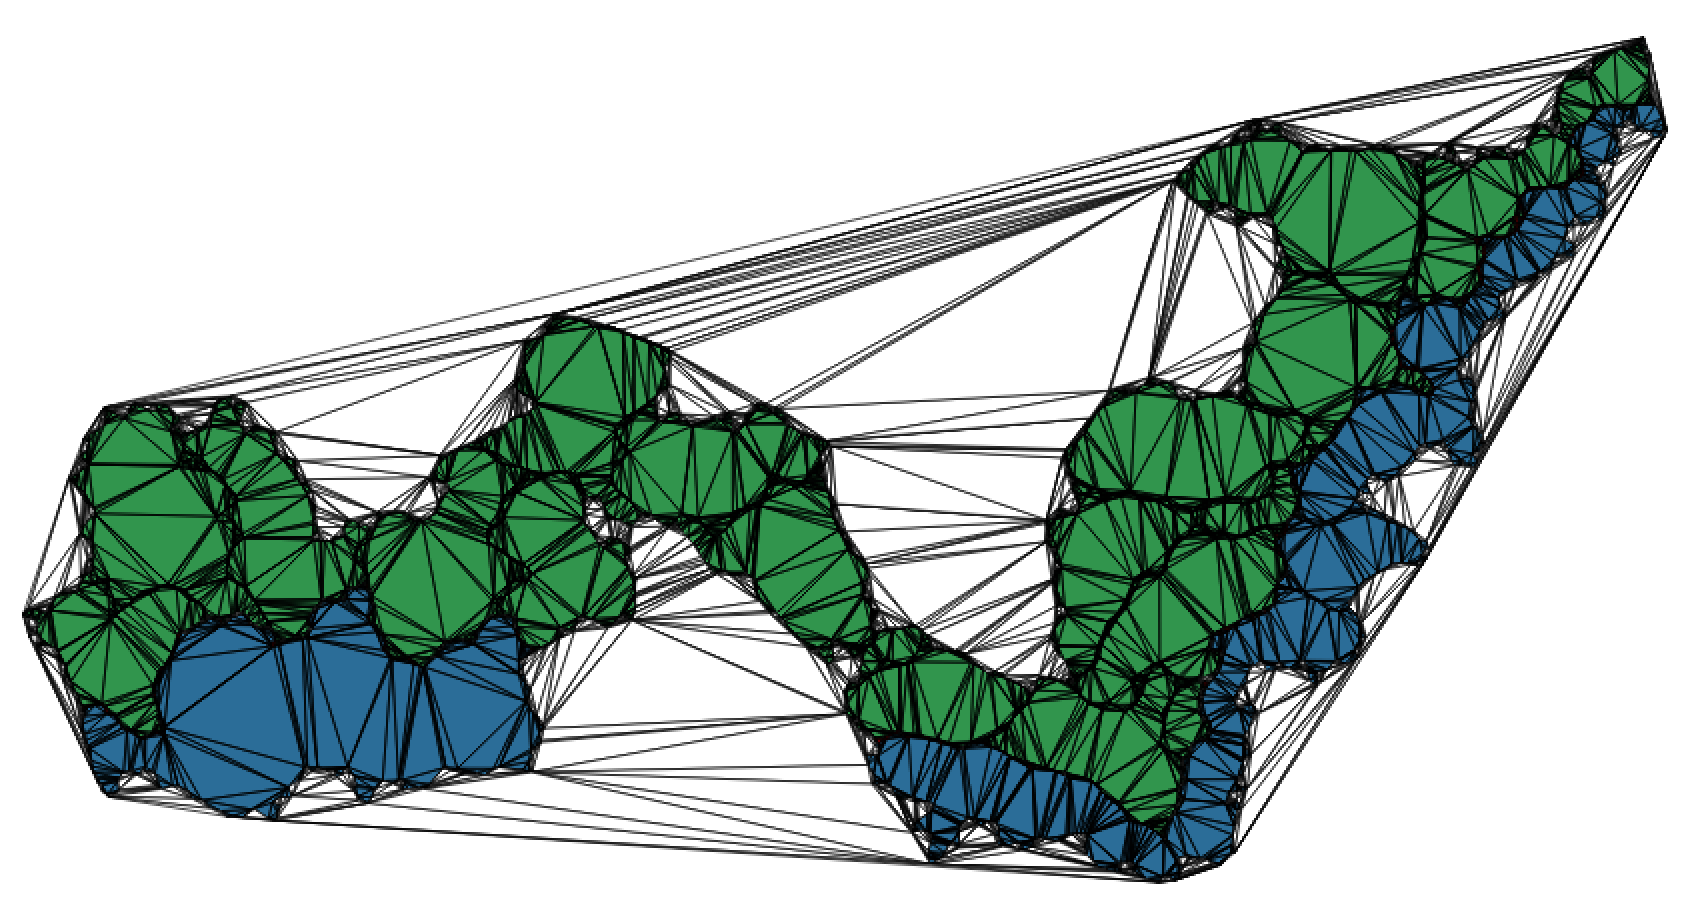
\includegraphics[width=\linewidth]{figs/sometriangles.png}
    \caption{}\label{fig:sidebyside:1}
  \end{subfigure}%
  \qquad %-- that adds some space between th 2 figures
  \begin{subfigure}[b]{0.45\linewidth}
    \centering
    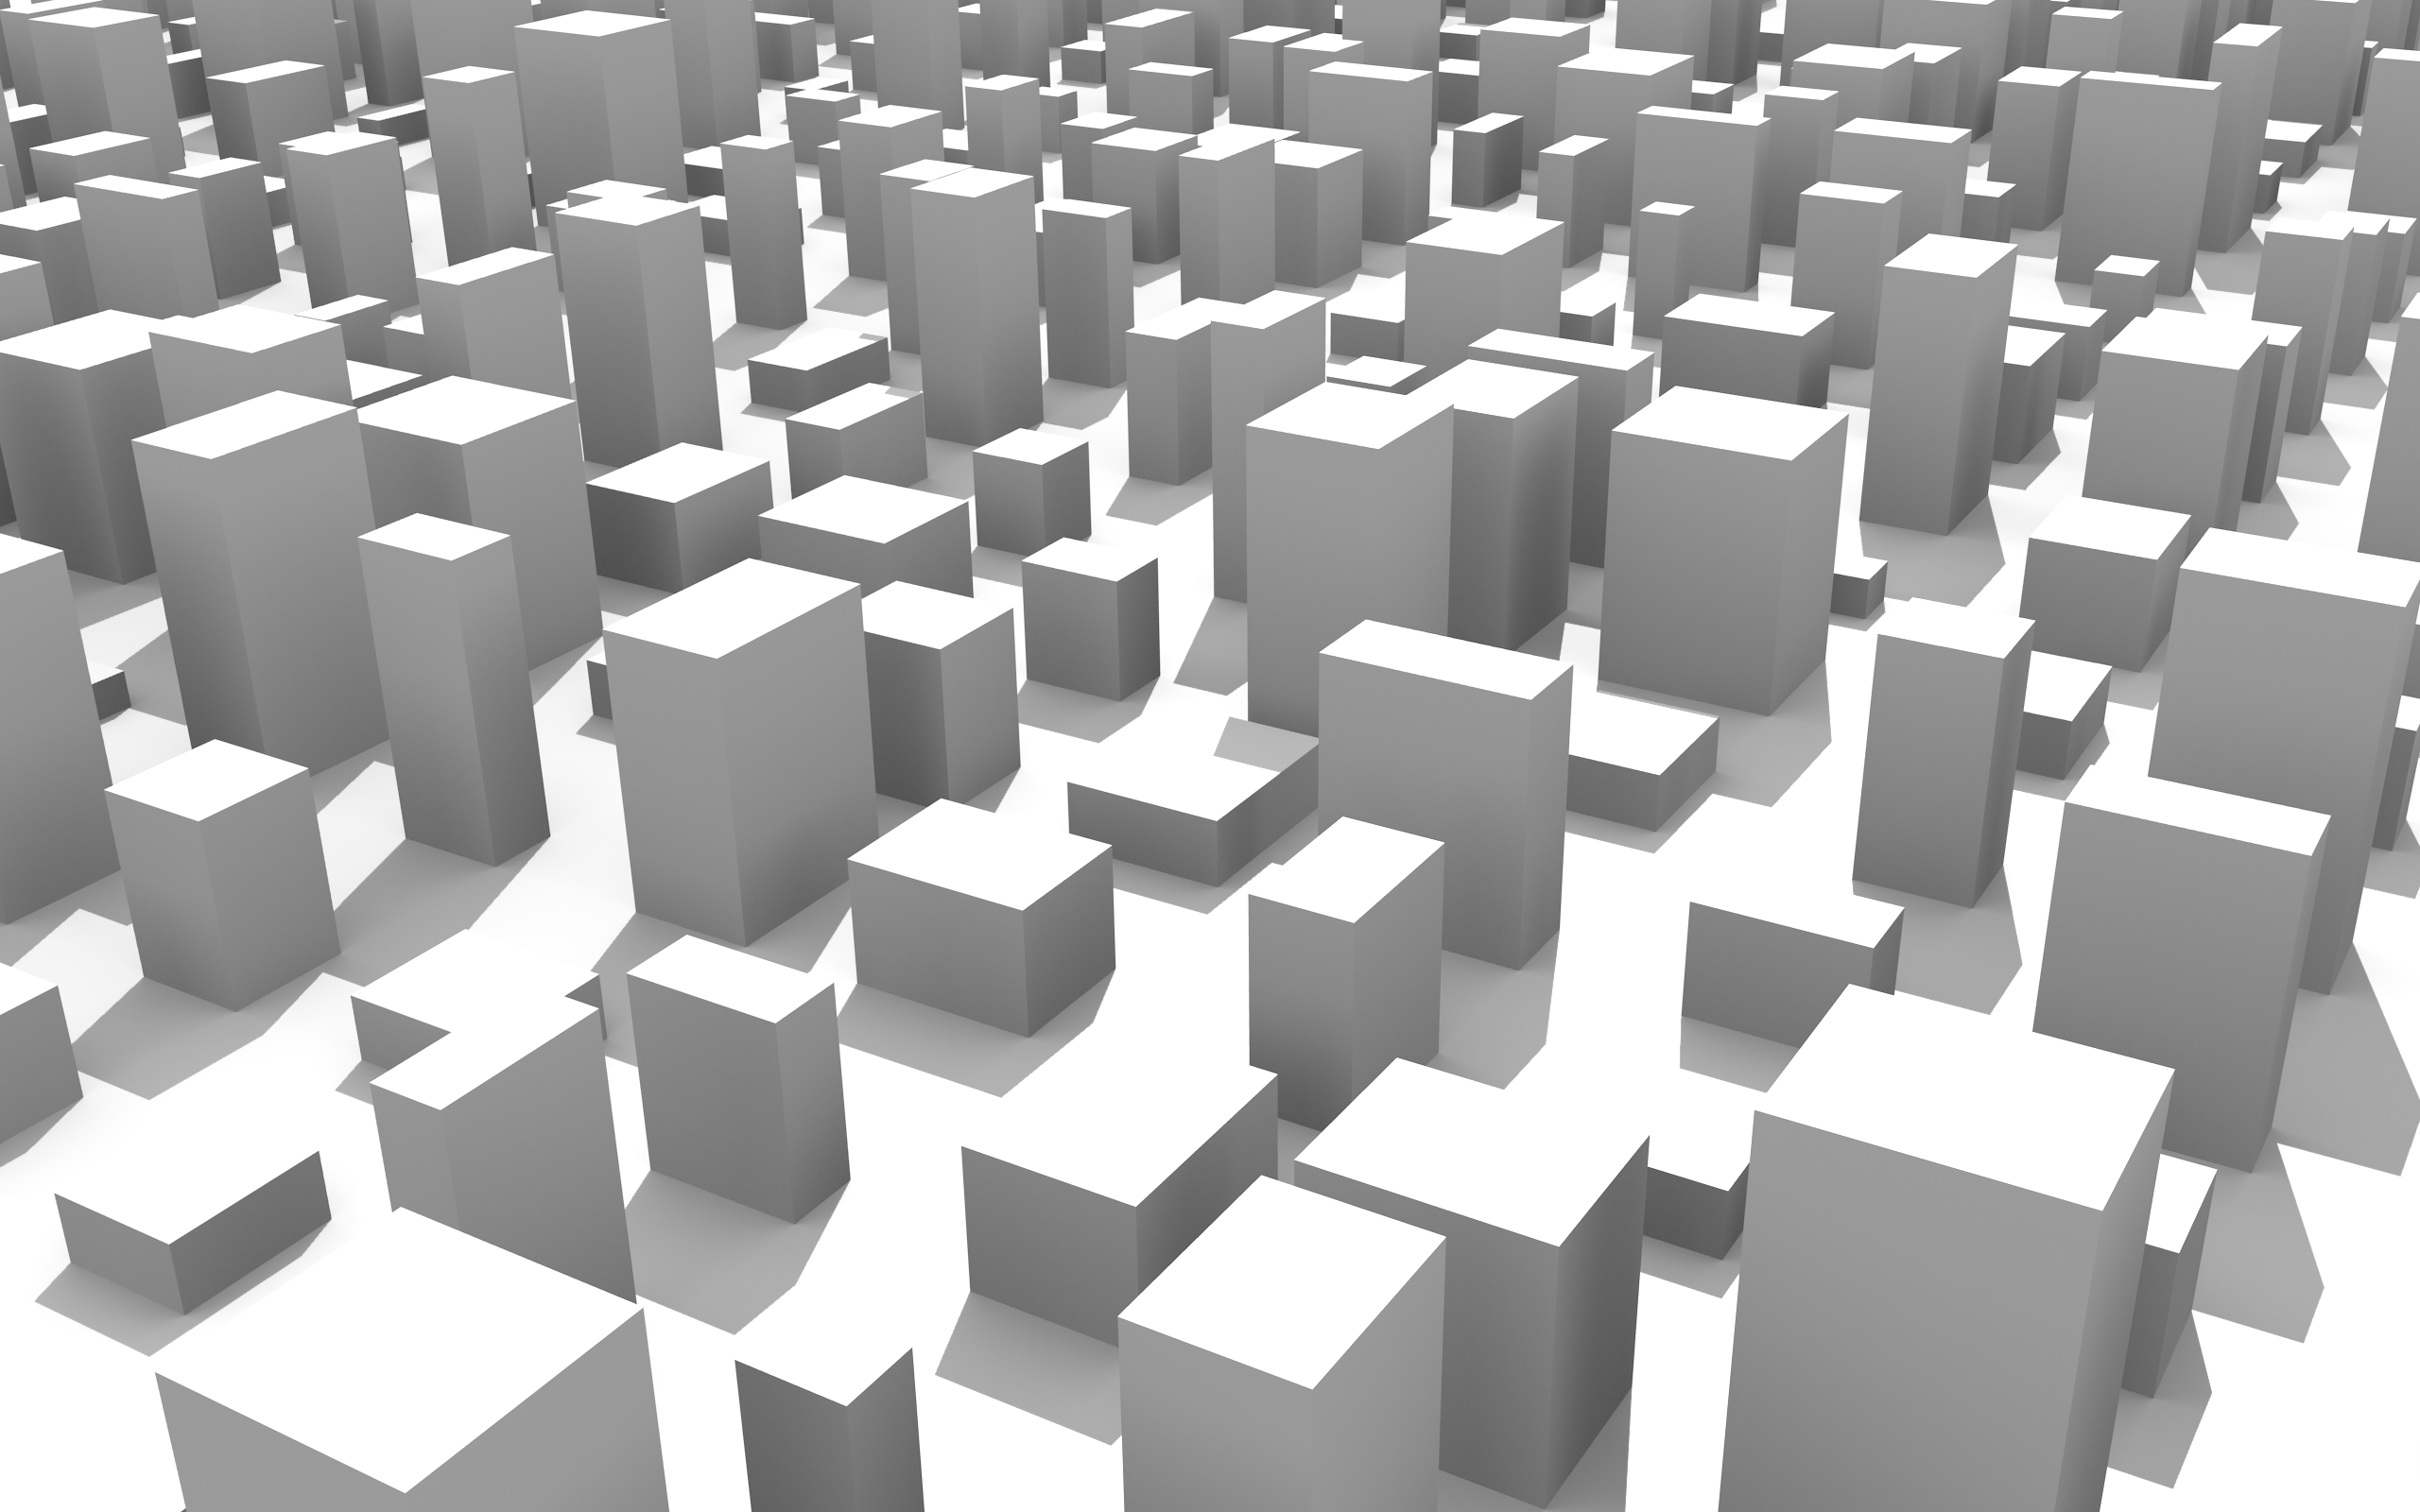
\includegraphics[width=\linewidth]{figs/lod1.png}
    \caption{}\label{fig:sidebyside:2}
  \end{subfigure}%
  \caption{Two figures side-by-side.}\label{fig:sidebyside}
\end{figure}
it is possible to have two figures (or more) side by side.
You can also refer to a subfigure: see Figure~\ref{fig:sidebyside:2}.


\subsection{Figures in PDF are possible (and better)}

If you use Adobe Illustrator or Ipe you can make your figures vectorial and save them in PDF\@.
You include a PDF the same way as you do for a PNG, see Figure~\ref{fig:pdffig},
\begin{figure}
  \centering
  \begin{subfigure}[b]{0.2\linewidth}
    \centering
    
\includegraphics[page=1,width=\linewidth]{figs/tricat.pdf}
    \caption{}\label{fig:pdffig:1}
  \end{subfigure}%
  \qquad %-- that adds some space between th 2 figures
  \begin{subfigure}[b]{0.2\linewidth}
    \centering
    
\includegraphics[page=2,width=\linewidth]{figs/tricat.pdf}
    \caption{}\label{fig:pdffig:2}
  \end{subfigure}%
  \qquad %-- that adds some space between th 2 figures
  \begin{subfigure}[b]{0.2\linewidth}
    \centering
    
\includegraphics[page=3,width=\linewidth]{figs/tricat.pdf}
    \caption{}\label{fig:pdffig:3}
  \end{subfigure}%
  \caption{Three PDF figures side-by-side.}\label{fig:pdffig}
\end{figure}



\section{How to add references?}

\citet{Descartes37} wrote and another one too~\citep{Voronoi08,Delaunay34}.


\section{Pseudo-code}

Please try to not put code (Python, C++, Fortran) in your thesis.
Put pseudo-code instead.
The package \texttt{algorithm2e} is pretty handy, see for instance the Algorithm~\ref{alg:myfirst}.
\begin{algorithm}[h]
 \KwData{this text}
 \KwResult{how to write algorithm with \LaTeX2e }
 initialization\;
 \While{not at end of this document}{
  read current\;
  \eIf{understand}{
   go to next section\;
   current section becomes this one\;
   }{
   go back to the beginning of current section\;
  }
 }
 \caption{How to write algorithms}\label{alg:myfirst}
\end{algorithm}
All your algorithms will be automatically added to the list of algorithms at the begining of the thesis.
